\begin{table}[t]
\centering
%\subtable[Twenty most frequent \emph{technical pairs} that are failure-related.]{
\begin{tabular}{@{\hspace{.2cm}}ccc@{\hspace{.75cm}}c@{\hspace{.2cm}}}
\toprule
Pair & \#successful & \#failed & $p_x$\\
\midrule
%Cody-Daisy&  0 & 12 & 1.0000 \\
%Adam-Ina & 0 & \phantom{1}8 & 1.0000 \\
%Adam-Kim& 0 & \phantom{1}8 & 1.0000 \\
%Adam-Nina & 0 & \phantom{1}6 & 1.0000 \\
%Fred-Gina& 0 & \phantom{1}6 & 1.0000 \\
%Gina-Oliver & 0 & \phantom{1}6 & 1.0000 \\
%Adam-Daisy& 1 & 14 & 0.9720\\%67 \\
%Bart-Daisy& 1 & \phantom{1}9 & 0.9572\\%127 \\
%Adam-Lisa& 1 & \phantom{1}8 & 0.9521\\%204 \\
%Bart-Eve & 2 & 11 & 0.9318\\%403 \\
%\textbf{Adam}-\textbf{Bart}& \textbf{3} & \textbf{13} & \textbf{0.9150}\\%485 \\
%Bart-Cody & 3 & 13 & 0.9150\\%485 \\
%Adam-Eve & 4 & 16 & 0.9086\\%162 \\
%Daisy-Ina & 3 & 12 & 0.9086\\%162 \\
%Cody-Fred& 3 & 10 & 0.8923\\%077 \\
%Bart-Herb & 3 & 10 & 0.8923\\%077 \\
%Cody-Eve & 5 & 15 & 0.8817\\%568 \\
%Adam-Jim & 4 & 11 & 0.8723\\%792 \\
%Herb-Paul & 5 & 12 & 0.8564\\%397 \\
%Mike-Rob& 6 & 13 & 0.8434\\%004\\
%Adam-Fred & 6 & 13 & 0.8434\\%004\\
%
%User11137, User4105 & 0 & 12 & 1.0000 \\
%User2943, User13877 & 0 & 8 & 1.0000 \\
%User7438, User2943 & 0 & 8 & 1.0000 \\
%User2943, User2810 & 0 & 6 & 1.0000 \\
%User8645, User1976 & 0 & 6 & 1.0000 \\
%User8645, User2267 & 0 & 6 & 1.0000 \\
%User11137, User2943 & 1 & 14 & 0.9675\\%908 \\
%User11137, User3493 & 1 & 9 & 0.9504\\%773 \\
%User6012, User2943 & 1 & 8 & 0.9446\\%298 \\
%User3493, User2435 & 2 & 11 & 0.9214\\%387 \\
%User3493, User2943 & 3 & 13 & 0.9023\\%53 \\
%User3493, User4105 & 3 & 13 & 0.9023\\%53 \\
%User2943, User2435 & 4 & 16 & 0.8950\\%695 \\
%User11137, User13877 & 3 & 12 & 0.8950\\%695 \\
%User1976, User4105 & 3 & 10 & 0.8766\\%716 \\
%User3493, User6339 & 3 & 10 & 0.8766\\%716 \\
%User4105, User2435 & 5 & 15 & 0.8648\\%208 \\
%User2943, User9017 & 4 & 11 & 0.8543\\%22 \\
%User6339, User13875 & 5 & 12 & 0.8365\\%498 \\
%User10979, User3385 & 6 & 13 & 0.8220\\%793\\
%User2943, User1976 & 6 & 13 & 0.8220\\%793 \\
%
(Cody, Daisy)	&	0&	12&	1		\\ %user11137.user4105.T
(Adam, Daisy)	&	1&	14&	0.9697	\\ %user11137.user2943.T
(Bart, Eve)	&	2&	11&	0.9265	\\ %user3493.user2435.T
(Adam, Bart)	&	3&	13&	0.9085	\\ %user3493.user2943.T
(Bart, Cody)	&	3&	13&	0.9085	\\ %user3493.user4105.T
(Adam, Eve)	&	4&	16&	0.9016	\\ %user2943.user2435.T
(Daisy, Ina)	&	3&	12&	0.9016	\\ %user11137.user13877.T
(Cody, Fred)	&	3&	10&	0.8843	\\ %user1976.user4105.T
(Bart, Herb)	&	3&	10&	0.8843	\\ %user3493.user6339.T
(Cody, Eve)	&	5&	15&	0.8730	\\ %user4105.user2435.T
(Adam, Jim)	&	4&	11&	0.8631	\\ %user2943.user9017.T
(Herb, Paul)	&	5&	12&	0.8462	\\ %user6339.user13875.T
(Cody, Fred)	&	5&	11&	0.8345	\\ %user11137.user1976.T
(Mike, Rob)	&	6&	13&	0.8324	\\ %user10979.user3385.T
(Adam, Fred)	&	6&	13&	0.8324	\\ %user2943.user1976.T
(Daisy, Fred)	&	8&	13&	0.7884	\\ %user3493.user1976.T
(Gill, Eve)		&	7&	10&	0.7661	\\ %user1264.user2435.T
(Daisy, Ina)	&	7&	10&	0.7661	\\ %user3493.user13873.T
(Fred, Ina)	&	8&	10&	0.7413	\\ %user1976.user13877.T
(Herb, Eve)	&	8&	10&	0.7413	\\ %user6339.user2435.T
\bottomrule
\end{tabular}
%\caption{Twenty \emph{technical pairs} that are failure-related and affect the most builds.}
%\label{tab:badtechpairs}
%}\hspace{1.3cm}
%\end{table}
%
%\subtable[The twenty corresponding \emph{socio-technical pairs}, which are not statistically related to failed builds.]{
%\begin{tabular}{@{\hspace{.2cm}}ccc@{\hspace{.75cm}}c@{\hspace{.2cm}}}
%\toprule
%Pair & \#successful & \#failed & $p_x$ \\
%\midrule
%(Cody, Daisy)	&	---&	---&	---\\
%(Adam, Daisy)	&	---&	---&	---\\
%(Bart, Eve)	&	1&	4&	0.9016\\
%(Adam, Bart)	&	---&	---&	---\\
%(Bart, Cody)	&	---&	---&	---\\
%(Adam, Eve)	&	---&	---&	---\\
%(Daisy, Ina)	&	---&	---&	---\\
%(Cody, Fred)	&	1&	0&	0\\
%(Bart, Herb)	&	1&	2&	0.8209\\
%(Cody, Eve)	&	0&	3&	1\\
%(Adam, Jim)	&	0&	1&	1\\
%(Herb, Paul)	&	1&	0&	0\\
%(Cody, Fred)	&	---&	---&	---\\
%(Mike, Rob)	&	---&	---&	---\\
%(Adam, Fred)	&	---&	---&	---\\
%(Daisy, Fred)	&	---&	---&	---\\
%(Gill, Eve)		&	---&	---&	---\\
%(Daisy, Ina)	&	1&	0&	0\\
%(Fred, Ina)	&	0&	2&	1\\
%(Herb, Eve)	&	---&	---&	---\\
%\bottomrule
%\end{tabular}
%%\caption{Twenty \emph{technical pairs} that are failure-related and affect the most builds.}
%\label{tab:stechpairs}
%}
\caption{The top 20 statistically failure related technical pairs.}
\label{tab:pairs}
\vspace{-20pt}
\end{table}




% \section{Pattern Analysis}
\section{Which Pairs Induce Failure?}
\label{sec:pattern}
In this section we answer our second research question, ``Are there
developer technical pairs that influence the build outcome?''. 
We first explain our analysis approach followed by the results obtained and a
short discussion of the results.

\subsection{Analysis of Socio-Technical Gaps}
The lack of communication between two developers that share a
technical dependency is referred to in the literature as a
socio-technical gap~\cite{valetto:msr:2007}. Because research suggests negative influence of such gaps, we are interested in analyzing pairs of developers that share a technical edge (implying coordination need) but no social edge (implying
unmet coordination need) in socio-technical networks. We refer to these pairs of
developers as \emph{technical pairs} (there is a gap), and to those that do
share a socio-technical edge (there is no gap) as \emph{socio-technical pairs}. 

To answer our second research question, we analyze the
technical pairs in relation to build
failure. Our analysis proceeds in four steps:

\begin{enumerate}
\item Identify all technical pairs from the socio-technical networks.
\item For each technical pair count occurrences in socio-technical networks of
failed builds.
\item For each technical pair count occurrences in socio-technical networks of
successful builds.
\item Determine if the pair is significantly related to success or failure.
\end{enumerate}

For example, in Table~\ref{tab:contingencytable} we illustrate the analysis of
the technical pair (Adam, Bart). This pair appears in 3 successful builds and in
13 failed builds. Thus it does not appear in 224 successful builds, which is the total number of successful builds minus the number of successful builds the pair appeared in, and it is absent in 86 failed builds.
A Fischer Exact Value test yields significance at a confidence level of $\alpha = .05$ with a p-value of $4.273\cdot10^{-5}$.

Note that we adjust the p-values of the Fischer Exact Value test to account for multiple hypothesis testing using the Bonferroni adjustment.
The adjustment is necessary because we deal with 961 technical pairs that need to be tested. 

To enable us to discuss the findings as to whether closing socio-technical gaps
are needed to avoid build failure, or which of these gaps are more important to
close, we peform two additional analyses. 
First we analyze whether the
socio-technical pairs also appear to be build failure-related or not, by
following the same steps as above for socio-technical pairs. 
%
Secondly, we prioritize the developer pairs using the coefficient $p_x$,
which represents the normalized likelihood of a build
to fail in the presence of the specific pair:

\begin{equation}
p_x\text{=}\frac{ \text{pair}_{failed} / \text{total}_{failed} }
                     { \text{pair}_{failed} / \text{total}_{failed} + \text{pair}_{success} / \text{total}_{successs}}
\end{equation}

The coefficient is comprised of four counts: (1) pair$_{failed}$, the number of failed builds where the pair occurred; (2) total$_{failed}$, the number of failed builds; (3) pair$_{success}$, the number of successful builds where the pair occurred; (4) total$_{success}$, the number of successful builds.
%This coefficient is normalized with the number of failed and successful builds.
A value closer to one means that the developer pair is strongly related to build
failure. %Additionally it describes a probability of failure likelihood that accounts for the imbalance in the data.

\addtocounter{table}{1}
\begin{table}[t]
\centering
\begin{tabular}{cccc}
\toprule
Feature & Coefficient & p-value & \\
\midrule
%(Intercept)             &  7.897e+74 & 3.743e+09 &  2.110e+65  &  <2e-16 & ***\\
%\\
%user11137.user4105.T    &   -5.669e+75  & 2.421e+10 &-2.342e+65 &  <2e-16 & ***\\
%user11137.user2943.T    &   -9.846e+75  &  7.788e+09 &-1.264e+66  & <2e-16 &***\\
%user3493.user2435.T      &    -1.258e+75      & 3.477e+10  &3.619e+64   &<2e-16 &***\\
%user3493.user2943.T      &    -1.605e+76     & 5.427e+10  &2.958e+65  & <2e-16 &***\\
%user3493.user4105.T      &   -3.419e+76     & 3.837e+10 &-8.910e+65  & <2e-16 &***\\
%user2943.user2435.T      &    -2.610e+76      & 2.966e+10  &8.801e+65  & <2e-16 &***\\
%user11137.user13877.T  &  -8.105e+74   & 3.036e+10 &-2.669e+64 &  <2e-16 &***\\
%user1976.user4105.T      &    -5.348e+76     & 2.359e+10  &2.267e+66   &<2e-16 &***\\
%user3493.user6339.T      &   -2.977e+76    &1.028e+11 &-2.895e+65   &<2e-16 &***\\
%user4105.user2435.T      &   -2.315e+76   & 1.618e+10 &-1.431e+66  & <2e-16 &***\\
%user2943.user9017.T      &    -2.724e+76    &2.621e+10  &1.039e+66  & <2e-16 &***\\
%user6339.user13875.T    &   -1.636e+76   & 4.081e+08 &-4.010e+67   &<2e-16 &***\\
%user11137.user1976.T    &   -1.645e+74   &4.024e+09 &-4.087e+64  & <2e-16 &***\\
%user10979.user3385.T    &    -1.327e+75   &3.668e+09  &3.619e+65  & <2e-16 &***\\
%user2943.user1976.T      &   -5.250e+76   &1.269e+10 &-4.136e+66  & <2e-16 &***\\
%user3493.user1976.T      &   -2.455e+75   & 3.523e+10 &-6.970e+64   &<2e-16 &***\\
%user1264.user2435.T      &    -7.162e+75   &3.589e+09  &1.996e+66  & <2e-16 &***\\
%user3493.user13873.T    &   -5.325e+74   & 3.464e+10 &-1.537e+64   &<2e-16 &***\\
%user1976.user13877.T    &    -2.777e+75   & 7.334e+08  &3.786e+66  & <2e-16 &***\\
%user6339.user2435.T      &    -1.799e+75   & 1.584e+09  &1.136e+66  & <2e-16 &***\\
%\\
%\#Change Sets per Build      & \phantom{-}6.480e+60 & 8.539e+06 & 7.589e+53 &  <2e-16 &***\\
%\#Files changed per Build             &-4.530e+60 & 3.072e+06 &-1.475e+54  & <2e-16 &***\\
%{\small \#Developers contributed per Build}  &   \phantom{-}3.386e+61 & 2.687e+07 & 1.260e+54 &  <2e-16 &***\\
%\#Work Items per Build     &  -3.690e+61 & 1.859e+07 &-1.984e+54  & <2e-16 &***\\
%
(Intercept)            &  7.897e+74 &  <2e-16 & ***\\
\\
(Cody, Daisy)  &  	-5.669e+75  &  <2e-16 & ***\\
(Adam, Daisy)  &   -9.846e+75  &   <2e-16 &***\\
(Bart, Eve)  	&   -1.258e+75  &<2e-16 &***\\
(Adam, Bart)  	&   -1.605e+76  & <2e-16 &***\\
(Bart, Cody)  	&   -3.419e+76  & <2e-16 &***\\
(Adam, Eve)  	&   -2.610e+76  & <2e-16 &***\\
(Daisy, Ina)  	&  	-8.105e+74 	 &  <2e-16 &***\\
(Cody, Fred)  	&   -5.348e+76  &<2e-16 &***\\
(Bart, Herb)  	&   -2.977e+76  &<2e-16 &***\\
(Cody, Eve)  	&   -2.315e+76  & <2e-16 &***\\
(Adam, Jim)  	&   -2.724e+76    & <2e-16 &***\\
(Herb, Paul)  	&   -1.636e+76      &<2e-16 &***\\
(Cody, Fred)  	&   -1.645e+74     & <2e-16 &***\\
(Mike, Rob)  	&   -1.327e+75    & <2e-16 &***\\
(Adam, Fred)  	&   -5.250e+76     & <2e-16 &***\\
(Daisy, Fred)  &   -2.455e+75      &<2e-16 &***\\
(Gill, Eve)	  	&   -7.162e+75    & <2e-16 &***\\
(Daisy, Ina)  	&   -5.325e+74      &<2e-16 &***\\
(Fred, Ina)  	&   -2.777e+75     & <2e-16 &***\\
(Herb, Eve)  	&   -1.799e+75     & <2e-16 &***\\
\\
\#Change Sets per Build     & \phantom{-}6.480e+60 &   <2e-16 &***\\
\#Files changed per Build            &-4.530e+60 &  <2e-16 &***\\
{\small \#Developers contributed per Build}  &   \phantom{-}3.386e+61 &  <2e-16 &***\\
\#Work Items per Build    &  -3.690e+61   & <2e-16 &***\\
%
%
%
%user6012.user2943.T     -1.198e+76  1.415e+10 -8.466e+65   <2e-16 ***\\
%user11137.user3493.T     4.917e+76  2.255e+10  2.180e+66   <2e-16 ***\\
%user2943.user13877.T    -2.086e+76  3.598e+10 -5.796e+65   <2e-16 ***\\
%user8645.user1976.T     -1.172e+75  4.535e+09 -2.585e+65   <2e-16 ***\\
%user8645.user2267.T      1.358e+76  2.934e+10  4.628e+65   <2e-16 ***\\
%user7438.user2943.T      1.562e+75  2.562e+10  6.096e+64   <2e-16 ***\\
%user10761.user9609.T    -1.244e+68  1.972e+08 -6.307e+59   <2e-16 ***\\
%user11208.user9017.T    -7.661e+73  6.520e+07 -1.175e+66   <2e-16 ***\\
%user11137.user8543.T    -7.938e+74  1.813e+08 -4.378e+66   <2e-16 ***\\
%user11281.user8543.T     1.520e+75  3.323e+09  4.573e+65   <2e-16 ***\\
%user3818.user8543.T     -1.655e+75  2.732e+10 -6.058e+64   <2e-16 ***\\
%user13877.user8543.T     1.802e+74  3.352e+09  5.377e+64   <2e-16 ***\\
%user9017.user13871.T    -3.613e+74  6.052e+09 -5.970e+64   <2e-16 ***\\
%user8645.user11281.T    -6.742e+73  1.058e+08 -6.371e+65   <2e-16 ***\\
%user2983.user9017.T     -6.303e+73  8.157e+09 -7.727e+63   <2e-16 ***\\
%user10979.user13875.T    1.507e+75  1.803e+10  8.355e+64   <2e-16 ***\\
%user9017.user13874.T    -2.791e+76  1.140e+11 -2.450e+65   <2e-16 ***\\
%user1264.user13874.T    -8.654e+75  2.838e+10 -3.049e+65   <2e-16 ***\\
%user3493.user9017.T     -2.786e+75  4.274e+09 -6.519e+65   <2e-16 ***\\
%user4105.user13874.T     1.206e+76  9.252e+10  1.303e+65   <2e-16 ***\\
%user2943.user13871.T    -6.665e+75  3.166e+10 -2.105e+65   <2e-16 ***\\
%user9017.user1976.T     -1.910e+63  3.850e+09 -4.960e+53   <2e-16 ***\\
%user10979.user2435.T     6.269e+63  3.579e+09  1.752e+54   <2e-16 ***\\
%user6639.user6339.T      3.075e+64  2.102e+10  1.463e+54   <2e-16 ***\\
%user6012.user9017.T     -5.463e+63  3.603e+09 -1.516e+54   <2e-16 ***\\
%user6339.user4105.T      5.169e+63  3.628e+09  1.425e+54   <2e-16 ***\\
%user9172.user2435.T     -1.212e+63  1.626e+09 -7.453e+53   <2e-16 ***\\
%user7438.user8543.T      5.042e+62  1.641e+09  3.073e+53   <2e-16 ***\\
%user11137.user13871.T    6.266e+62  5.193e+08  1.207e+54   <2e-16 ***\\
%user10979.user11281.T   -5.506e+63  3.719e+09 -1.480e+54   <2e-16 ***\\
%user11137.user6012.T     2.332e+63  1.532e+09  1.522e+54   <2e-16 ***\\
%user11137.user13874.T   -1.913e+64  1.393e+10 -1.373e+54   <2e-16 ***\\
%user1264.user4105.T      1.212e+63  1.420e+09  8.533e+53   <2e-16 ***\\
%user8645.user6096.T      6.633e+63  4.523e+09  1.467e+54   <2e-16 ***\\
%user11281.user9609.T     5.157e+62  7.503e+07  6.873e+54   <2e-16 ***\\
%user13871.user4163.C     8.406e+61  1.717e+08  4.897e+53   <2e-16 ***\\
%user11840.user9172.C    -1.672e+61  4.148e+08 -4.031e+52   <2e-16 ***\\
%user11840.user9983.C     2.743e+62  2.898e+08  9.463e+53   <2e-16 ***\\
%user6727.user9983.C      1.659e+63  1.698e+09  9.771e+53   <2e-16 ***\\
%user11208.user6727.C    -2.455e+63  1.596e+09 -1.538e+54   <2e-16 ***\\
%user3057.user13873.C     1.983e+62  1.260e+08  1.574e+54   <2e-16 ***\\
%user11137.user11208.C   -9.030e+61  2.237e+08 -4.036e+53   <2e-16 ***\\
%user3982.user6012.C     -2.567e+62  3.356e+08 -7.648e+53   <2e-16 ***\\
%user3818.user10979.C     1.868e+62  1.228e+08  1.522e+54   <2e-16 ***\\
%user6012.user9172.C      1.353e+62  1.089e+08  1.242e+54   <2e-16 ***\\
%user13877.user13875.C   -1.013e+63  6.884e+08 -1.472e+54   <2e-16 ***\\
%user11208.user7438.C     8.180e+61  8.746e+07  9.353e+53   <2e-16 ***\\
%user10979.user6096.C    -5.291e+63  3.648e+09 -1.450e+54   <2e-16 ***\\
%user6096.user7395.C     -3.135e+61  1.839e+08 -1.705e+53   <2e-16 ***\\
%user4105.user5275.C      2.725e+63  9.779e+08  2.787e+54   <2e-16 ***\\
%user7146.user4163.C      1.171e+63  5.291e+08  2.214e+54   <2e-16 ***\\
%user11208.user2267.C     3.459e+61  3.525e+08  9.813e+52   <2e-16 ***\\
%user7224.user4163.C      2.375e+61  1.379e+08  1.723e+53   <2e-16 ***\\
%user13877.user2435.C     2.353e+63  1.838e+09  1.280e+54   <2e-16 ***\\
%user6012.user7146.C     -6.092e+62  2.884e+08 -2.112e+54   <2e-16 ***\\
%user2983.user7224.C      2.961e+61  1.340e+08  2.209e+53   <2e-16 ***\\
%user13235.user1976.C     7.225e+63  5.490e+09  1.316e+54   <2e-16 ***\\
%user11208.user7372.C     5.809e+63  3.983e+09  1.458e+54   <2e-16 ***\\
%user13235.user13874.C    5.605e+63  3.718e+09  1.507e+54   <2e-16 ***\\
%user3057.user13874.C     5.278e+63  3.817e+09  1.383e+54   <2e-16 ***\\
%user11208.user6012.C     4.458e+61  1.043e+08  4.273e+53   <2e-16 ***\\
%user7002.user2020.C     -5.853e+63  3.978e+09 -1.471e+54   <2e-16 ***\\
%user2744.user11208.C     7.773e+62  7.092e+08  1.096e+54   <2e-16 ***\\
%user9172.user5275.C      1.397e+64  9.128e+09  1.530e+54   <2e-16 ***\\
%user6677.user7224.C      2.952e+61  1.316e+08  2.244e+53   <2e-16 ***\\
%user3818.user6639.C      5.573e+61  2.800e+08  1.991e+53   <2e-16 ***\\
%user7002.user4105.C     -2.017e+63  9.206e+08 -2.191e+54   <2e-16 ***\\
%user12149.user2943.C    -1.655e+64  9.635e+09 -1.718e+54   <2e-16 ***\\
%user7438.user7372.C     -9.768e+61  2.375e+08 -4.113e+53   <2e-16 ***\\
%user4955.user2306.C     -4.290e+62  4.334e+08 -9.898e+53   <2e-16 ***\\
%user11137.user7438.C    -8.275e+61  7.426e+08 -1.114e+53   <2e-16 ***\\
%user11208.user7002.C     1.709e+62  8.605e+07  1.986e+54   <2e-16 ***\\
%user3057.user1976.C      3.156e+60  4.486e+08  7.034e+51   <2e-16 ***\\
%user3982.user4163.C     -1.497e+63  7.778e+08 -1.925e+54   <2e-16 ***\\
%user10761.user4105.C     5.332e+62  3.087e+08  1.727e+54   <2e-16 ***\\
%user7438.user6639.C     -4.700e+62  1.319e+08 -3.564e+54   <2e-16 ***\\
%user10761.user6339.C     8.421e+61  1.068e+08  7.887e+53   <2e-16 ***\\
%user7438.user2267.C      5.206e+62  8.470e+07  6.146e+54   <2e-16 ***\\
%user11840.user2267.C    -1.418e+62  3.676e+08 -3.858e+53   <2e-16 ***\\
%user3057.user4163.C      5.427e+63  3.853e+09  1.409e+54   <2e-16 ***\\
%user11208.user6639.C     6.044e+62  6.502e+08  9.295e+53   <2e-16 ***\\
%user6012.user4163.C      4.410e+61  9.535e+07  4.625e+53   <2e-16 ***\\
%user6677.user6379.C      1.691e+61  1.481e+08  1.142e+53   <2e-16 ***\\
%user10761.user3639.C    -1.635e+62  1.878e+08 -8.709e+53   <2e-16 ***\\
%user9655.user10979.C    -1.393e+61  8.225e+07 -1.693e+53   <2e-16 ***\\
%user4955.user9986.TC     5.594e+61  8.556e+07  6.538e+53   <2e-16 ***\\
%user4105.user1567.C      1.454e+62  9.109e+07  1.596e+54   <2e-16 ***\\
%user9609.user6012.T      5.290e+61  1.824e+08  2.900e+53   <2e-16 ***\\
%user11281.user2267.T    -5.499e+63  3.725e+09 -1.476e+54   <2e-16 ***\\
%user2983.user8860.C      3.596e+62  1.531e+08  2.349e+54   <2e-16 ***\\
%user3672.user13875.C    -6.807e+61  1.880e+08 -3.621e+53   <2e-16 ***\\
%user2452.user9983.C     -3.179e+62  3.396e+08 -9.359e+53   <2e-16 ***\\
%user3756.user7372.C      7.300e+61  5.508e+07  1.325e+54   <2e-16 ***\\
%user3539.user13877.C     4.104e+62  1.941e+08  2.114e+54   <2e-16 ***\\
%user2460.user6103.C      8.697e+61  3.716e+08  2.340e+53   <2e-16 ***\\
%user6021.user9017.C      1.049e+62  7.032e+07  1.491e+54   <2e-16 ***\\
%user6901.user2038.T      2.862e+61  9.837e+07  2.909e+53   <2e-16 ***\\
%user6677.user5963.C      9.236e+60  7.371e+07  1.253e+53   <2e-16 ***\\
%user10761.user6677.C    -4.323e+62  4.038e+08 -1.071e+54   <2e-16 ***\\
%user13874.user11208.C   -5.371e+63  3.581e+09 -1.500e+54   <2e-16 ***\\
%user3982.user2943.C     -6.644e+61  2.197e+08 -3.024e+53   <2e-16 ***\\
%user3057.user7286.C     -2.138e+60  1.090e+08 -1.962e+52   <2e-16 ***\\
%user7111.user11623.C     1.263e+63  5.111e+08  2.471e+54   <2e-16 ***\\
%user9983.user6677.C      3.487e+62  3.489e+08  9.995e+53   <2e-16 ***\\
%user7438.user6677.TC    -5.068e+63  3.650e+09 -1.388e+54   <2e-16 ***\\
%user11281.user7438.C     2.607e+61  9.562e+07  2.726e+53   <2e-16 ***\\
%user4686.user6391.C      3.592e+62  1.623e+08  2.214e+54   <2e-16 ***\\
%user10303.user4105.C     9.159e+61  7.919e+07  1.157e+54   <2e-16 ***\\
%user4955.user3818.C      1.993e+62  1.600e+08  1.246e+54   <2e-16 ***\\
%user13871.user6391.C    -1.917e+62  2.296e+08 -8.351e+53   <2e-16 ***\\
%user11137.user3818.T    -1.882e+62  1.920e+08 -9.800e+53   <2e-16 ***\\
%user9609.user11281.TC   -1.094e+62  1.955e+08 -5.596e+53   <2e-16 ***\\
%user6677.user6639.C     -4.807e+63  3.646e+09 -1.319e+54   <2e-16 ***\\
%user7689.user7286.C      2.220e+60  7.506e+07  2.958e+52   <2e-16 ***\\
%user7438.user7689.T     -1.661e+62  1.214e+08 -1.368e+54   <2e-16 ***\\
%user6677.user2810.C     -2.554e+60  6.772e+07 -3.771e+52   <2e-16 ***\\
%user1077.user13871.C    -1.468e+61  8.322e+07 -1.764e+53   <2e-16 ***\\
%user11208.user13871.T   -6.376e+61  1.523e+08 -4.187e+53   <2e-16 ***\\
%user6639.user11281.C    -1.021e+62  8.631e+07 -1.183e+54   <2e-16 ***\\
%user6677.user6727.C     -8.135e+61  1.169e+08 -6.959e+53   <2e-16 ***\\
%user10761.user1264.C    -9.014e+60  2.694e+08 -3.346e+52   <2e-16 ***\\
%user2452.user2983.C      6.650e+61  9.949e+07  6.685e+53   <2e-16 ***\\
%user11281.user7438.TC    2.085e+62  7.164e+07  2.910e+54   <2e-16 ***\\
%user1264.user2943.C     -1.568e+62  1.711e+08 -9.162e+53   <2e-16 ***\\
%user6339.user7689.T      3.002e+62  1.879e+08  1.597e+54   <2e-16 ***\\
%user10517.user11840.C   -5.510e+63  3.837e+09 -1.436e+54   <2e-16 ***\\
%user7438.user6677.C      2.349e+61  7.951e+07  2.955e+53   <2e-16 ***\\
%user3057.user6021.C     -5.461e+61  5.719e+07 -9.548e+53   <2e-16 ***\\
%user11137.user2038.C    -7.344e+61  1.607e+08 -4.570e+53   <2e-16 ***\\
%user6727.user2983.C      3.770e+61  1.191e+08  3.165e+53   <2e-16 ***\\
%user11281.user10849.C   -4.757e+61  1.248e+08 -3.812e+53   <2e-16 ***\\
%user6021.user5275.C      1.601e+62  1.424e+08  1.124e+54   <2e-16 ***\\
%user6339.user11281.TC    5.532e+63  3.717e+09  1.488e+54   <2e-16 ***\\
%user3982.user9172.C      2.099e+62  1.581e+08  1.328e+54   <2e-16 ***\\
%user7146.user3818.C      2.601e+60  8.291e+07  3.137e+52   <2e-16 ***\\
%user11208.user8543.T    -4.465e+61  8.689e+07 -5.139e+53   <2e-16 ***\\
%user10979.user3539.C     1.514e+61  8.288e+07  1.826e+53   <2e-16 ***\\
%user8645.user11281.C     1.372e+62  4.692e+07  2.924e+54   <2e-16 ***\\
%user11281.user7002.C    -1.453e+61  4.487e+07 -3.238e+53   <2e-16 ***\\
%user3982.user7146.C      1.576e+62  1.342e+08  1.174e+54   <2e-16 ***\\
%user9983.user7689.C     -5.070e+63  3.610e+09 -1.404e+54   <2e-16 ***\\
%user2452.user6215.C      3.324e+61  6.875e+07  4.836e+53   <2e-16 ***\\
%user11281.user9609.C     1.806e+61  6.370e+07  2.835e+53   <2e-16 ***\\
%user11281.user2983.C    -2.505e+61  8.608e+07 -2.910e+53   <2e-16 ***\\
%user11208.user11840.C    6.661e+61  1.573e+08  4.236e+53   <2e-16 ***\\
%user7224.user9609.C      6.556e+61  1.029e+08  6.374e+53   <2e-16 ***\\
%user13875.user13871.C   -1.769e+62  2.469e+08 -7.166e+53   <2e-16 ***\\
%user11281.user1227.C     1.188e+61  7.815e+07  1.520e+53   <2e-16 ***\\
%user6037.user11281.C     5.378e+61  3.069e+07  1.752e+54   <2e-16 ***\\
%user2435.user6012.T      2.009e+62  8.135e+07  2.470e+54   <2e-16 ***\\
%user11281.user3818.C     1.975e+61  2.844e+07  6.942e+53   <2e-16 ***\\
%user11281.user6677.C     9.267e+61  8.526e+07  1.087e+54   <2e-16 ***\\
%user6339.user9017.C      5.143e+61  4.972e+07  1.035e+54   <2e-16 ***\\
%user2038.user3756.C      1.465e+58  9.491e+07  1.544e+50   <2e-16 ***\\
%user8860.user10623.C     2.737e+61  7.109e+07  3.850e+53   <2e-16 ***\\
%user7438.user7146.C     -5.663e+60  9.529e+07 -5.943e+52   <2e-16 ***\\
%user10433.user5564.C    -2.747e+61  1.538e+08 -1.787e+53   <2e-16 ***\\
%user6677.user11281.T    -2.151e+62  7.131e+07 -3.016e+54   <2e-16 ***\\
%user11281.user3057.C     2.576e+61  4.683e+07  5.502e+53   <2e-16 ***\\
%user9609.user6677.C      2.740e+60  9.492e+07  2.887e+52   <2e-16 ***\\
%user6677.user10899.TC    8.748e+60  1.528e+08  5.724e+52   <2e-16 ***\\
%
%
\bottomrule
\end{tabular}
\caption{Logistic regression only showing the technical pairs from Table~\ref{tab:badtechpairs}, the intercept, and the confounding variables, the model reaches an AIC of 7006 with all shown features being significant at $\alpha=0.001$ level (indicated by ***).}
\label{tab:regression}
\end{table}

\subsection{Results}
We found a total of 2872 developer pairs in all the constructed
socio-technical networks, out of which 961 were technical pairs. %. The Fischer Exact Value tests show While a Fischer Exact Value test determined 120 technical pairs that are significantly correlated with build failure, none are statistically related with successful builds. Due to space constraints we display only twenty pairs in Table~\ref{tab:badtechpairs}.
We choose to present the twenty that are most frequent across failed builds.

We rank the failure relating \emph{technical} pairs (see Tables~\ref{tab:badtechpairs})
by the coefficient $p_{x}$. This coefficient indicates the strength of
relationship between the developer pair and build failure. For instance, the
developer pair (Adam, Bart), appears in 13 failed builds and in 3
successful builds. This means that pair$_{failed}$ = 13 and pair$_{success}$ = 3
with total$_{failed}$= 99 and total$_{success}$= 227 result in $p_x$= 0.9016.
Besides that we report the number of successful builds the pair was observed with
(\#successful) as well as the number of failed builds the pairs was observed with
(\#failed). The $p_x$ values are all above 0.74, implying that the likelihood
of failure is at least 74\% in all builds in which these developers pairs are
involved. 

We then checked for the 120 pairs whether the corresponding \emph{socio-technical} pairs are related to failure.
Only 23 of the 120 technical pairs had an existing corresponding socio-technical pair of which none were statistically related to build failure. 
In Table~\ref{tab:stechpairs} we show the socio-technical pairs that match the 20 technical pairs shown in Table~\ref{tab:badtechpairs} as well as the same information as in Table~\ref{tab:badtechpairs}.
If the corresponding socio-technical pair existed we computed the same statistics as for the technical pairs, but for those that existed we could not find statistical significance.
Note that we use fictitious names for confidentiality reasons.

The failure-related technical pairs span 48 out of the total 99 failed builds in
the project. Figure~\ref{fig:builddistribution} shows their distribution
 across the 48 failed builds. The histogram
illustrates that there are few builds that have a large number of failure related
builds, e.g. 4 with 18 or more pairs, but most builds only show a small number of
pairs (15 out of 48 failed builds have 4 or less). 
%Not only does 
This distribution of technical pairs indicate that the developer
pairs we found  did not concentrate in a small number of builds. 
In addition, it validates the assumption that it is
worthwhile seeking insights about developer coordination in failed builds.
%Moreover, this enables us to explain why two thirds of the builds failed.


\begin{figure}[t]
\centering
\vspace{-1cm}
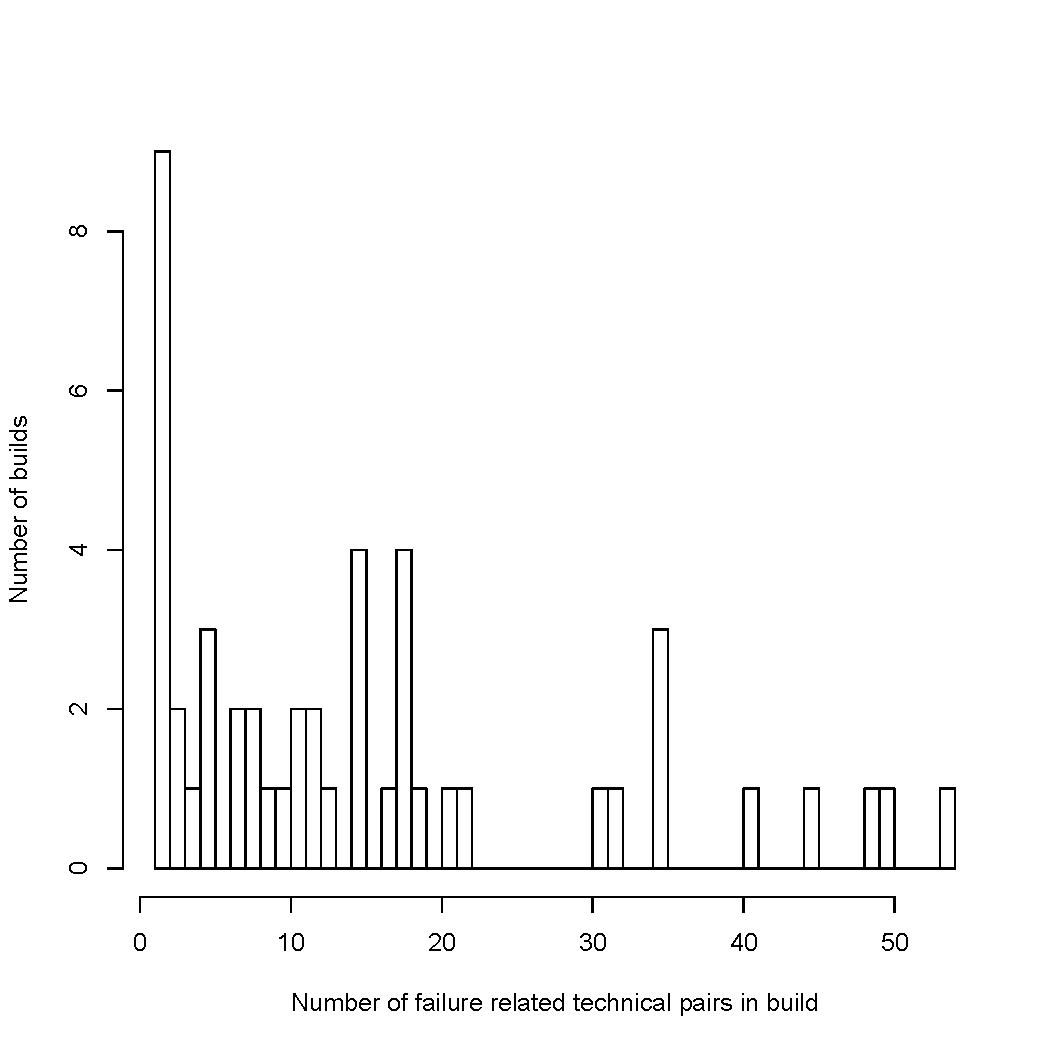
\includegraphics[width=\columnwidth]{builddistribution}
\vspace{-.75cm}
\caption{Histogram plotting how many builds have a certain number of failure-reated technical pairs.}
\label{fig:builddistribution}
\end{figure}

\subsection{Discussion}
% answered the the research question
These results show that there is a strong relationship between certain technical
developer pairs and increased likelihood of a build failure.
% meaning of patterns
Out of the total of 120 technical pairs that increase the likelihood of a
build to fail, only 23 had an existing
corresponding socio-technical pair. Of these, none were statistically
related to build failure. This means that 97 pairs of developers that had a
technical dependency did not communicate with each other and
consequently increased the likelihood of a build failure. Our results not only
corroborate past findings~\cite{cataldo:cscw:2006,cataldo:esem:2008} that socio-technical gaps
have a negative effect in software development. More importantly, they indicate
that the analysis presented in this paper is able to identify the specific
socio-technical gaps, namely the actual developer pairs where the gaps occur
and that increase the likelihood of build failure. 

% contrast of t and st patterns After investigating the pairs closer with respect
% to team allocation, we found that most of the pairs span do not originate from
% the same team.
Although not a goal of this paper, we sought possible explanations for the
socio-technical gaps in this project. A preliminary analysis of developers
membership to teams shows that most
of the technical pairs related to build failure consist of developer belonging to
different teams. Naggappan et al.~\cite{nagappan:icse:2008} found that using the
organizational distance between people predicts failures. They reasoned that this
is due to the lack of awareness what people separated by organizational distance
work on. Although the Jazz team strongly emphasizes communication
regardless of team boundaries, it still seems that organizational distance has
an influence on its communication behavior.

% bridge to regression - confounding variables?
Further, although the analysis of technical pairs in relation to build failures
showed that they have a negative influence on the build result, it does not take
into account possible confounding variables. The question is if there developer pairs still effect the build outcome in the presence of confounding variables, such as number of developers involved in a build, number of work items
related to a build, number of change sets per build, and number of files changed.
We tested this using a logistical regression model including both developer pairs and confounding variables.

Overall the logistic regression confirms the effect of the developer pairs
even in the presence of confounding variables, such as number of files changed
and numbers of developers (AIC of 7006). 
Table~\ref{tab:regression} shows an excerpt from the complete logistical
regression which shows that the twenty pairs previously identified are still
significant under the influence of the four confounding variables. Because we have 2872 developer pairs, space constraints prevent us from reporting the entire regression model. We chose to report on the coefficients for the twenty pairs that we reported in Table~\ref{tab:regression} as well as the coefficients for the four control features.

All features shown in Table~\ref{tab:regression} are significant at the $\alpha=.001$ level (indicated by the p-value and ***).
We checked for all the other technical pairs that were reported significant using the approach described in the previous section and found that they are all significant in the regression model as well.
Moreover, the four control variables of number of developers per build, number
of work items per build, number of change sets per build, and number of files changed per build are also significant.

% explain the coefficient interpretation
% some of the pairs are positive
% some are negative
% extreme magnitude
Since we model failed builds with 0 and successful builds with 1, a negative coefficient means that the feature increases the chances of a failure.
All pairs reported in Table~\ref{tab:regression} and the technical pairs that we identified to be related to build failure have a negative coefficient.
 
% about the control variables
%As shown in Table~\ref{tab:regression} two of the four control features, number of change sets per build and number of developers contributing to a build increase the likelihood of a build succeeding.
%On the other hand number of files changed per build and number of work items per build increase the likelihood of a build failing.

In conclusion, we can answer our second research question with yes: there are
certain technical pairs that are significantly related to build failure, and
this happens even in the presence of possibly confounding variables. 




